\chapter[Leçon 38: D'Thema Musek, Modalverben a Sazbau]{Leçon 38: D'Thema Musek, Sproochentest-Virbereedung, Modalverben a Sazbau}

Dës Lektioun baséiert op engem interaktiven a liewege Cours vum 24. Oktober 2026. Mir behandele fundamental Strukture fir d'Alldagskommunikatioun an eng geziilt Virbereedung op den mëndlechen Deel vum \textbf{Sproochentest Lëtzebuergesch}. De Schwéierpunkt läit op dem Thema \textbf{Musek} (Museksgoût, Liiblingskënschtler, Instrumenter spillen, Concerten a Festivaller zu Lëtzebuerg). Donieft ënnersiche mir typesch däitsch \textit{Faux-amis} (firwat et \textit{welche} am Lëtzebuergeschen net gëtt a firwat een \textit{eppes} amplaz vun \textit{etwas} seet), d'Ënnerscheeder tëscht \textit{héieren} a \textit{lauschteren}, komplex Sazkonstruktioune mat Niewesätz (\textit{Wann...}) a Reflexivverben (\textit{sech langweilen}), d'Benotzung vun de \textbf{Modalverben am Präteritum} (\textit{konnt}, \textit{wollt}, \textit{sollt}, \textit{musst}, \textit{duerft}, \textit{wousst}), Zäitausdréck an d'Eifeler Regel.

\textit{Cette leçon est consacrée à des structures fondamentales de la communication courante et constitue une préparation ciblée à l'épreuve orale du \textbf{Sproochentest}. Le thème central est la \textbf{musique} (goûts musicaux, artistes préférés, pratique d'un instrument, concerts et salles de spectacle au Luxembourg). Nous analysons également des faux-amis fréquents issus de l'allemand (l'absence de \textit{welche} au profit de \textit{wat fir eng}, l'usage d'\textit{eppes} au lieu d'\textit{etwas}), la distinction entre \textit{héieren} (entendre) et \textit{lauschteren} (écouter), la construction de propositions subordonnées complexes (\textit{Wann...}) combinées à des verbes pronominaux (\textit{sech langweilen}) et l'inversion du sujet, l'emploi systématique des \textbf{verbes modaux au prétérit} (\textit{konnt}, \textit{wollt}, \textit{sollt}, \textit{musst}, \textit{duerft}, \textit{wousst}), l'axe temporel et l'application de la règle de l'Eifel (\textit{Eifeler Regel}).}

\textit{This lesson is based on the interactive class of October 24, 2026, and provides comprehensive preparation for the oral component of the \textbf{Sproochentest}. The core focus is on the topic of \textbf{music} (musical tastes, favorite artists, playing instruments, attending concerts and music venues in Luxembourg). We also address key Luxembourgish-German contrasts (the absence of \textit{welche} replaced by \textit{wat fir eng}, using \textit{eppes} instead of \textit{etwas}), the contrast between \textit{héieren} (to hear) and \textit{lauschteren} (to listen), complex subordinate clauses with \textit{Wann...} combined with reflexive verbs (\textit{sech langweilen}) and subject-verb inversion (V2 rule), the essential use of \textbf{modal verbs in the preterite} (\textit{konnt}, \textit{wollt}, \textit{sollt}, \textit{musst}, \textit{duerft}, \textit{wousst}), temporal adverbs and future expression in spoken Luxembourgish, and the Eifeler Regel.}

\vspace{1.5em}

% ==============================================================================
% SECTION I: THEMA MUSEK
% ==============================================================================
\section[D'Thema Musek am Alldag an am Sproochentest / Topic: Music]{D'Thema Musek am Alldag an am Sproochentest \\/ Le thème de la musique au quotidien et au Sproochentest \\/ The Topic of Music in Everyday Life and the Sproochentest}

D'Thema Musek gehéiert zu de beléiftste Sujeten am mëndlechen Deel vum Sproochentest. Et erlaabt Iech, Är perséinlech Virléiften ze beschreiwen, iwwer Är Fräizäit ze schwätzen a reegelméisseg Gewunnechten auszedrécken. \\
\textit{FR : Le thème de la musique compte parmi les sujets les plus fréquents de l'épreuve orale du Sproochentest. Il vous permet de décrire vos préférences personnelles, d'évoquer vos loisirs et d'exprimer vos habitudes régulières.} \\
\textit{EN : The topic of music is one of the most popular subjects in the oral section of the Sproochentest. It allows you to describe your personal preferences, discuss your leisure time, and express regular habits.}

\subsection{Froen an Äntwerten iwwer de Museksgoût / Parler de ses goûts musicaux / Discussing Music Tastes}

Wann Dir Iech iwwer Musek ënnerhaalt, ginn et typesch Froen an Äntwerten, déi Dir automatiséiere sollt : \\
\textit{FR : Lorsque vous parlez de musique, il y a des questions et réponses types que vous devriez automatiser :} \\
\textit{EN : When discussing music, there are typical questions and answers that you should automate:}

\begin{itemize}
    \item \textbf{Fro no der Museksrichtung / Demander le genre musical / Asking about music genres :}
    \begin{itemize}
        \item \textit{Informell (Duzen / tutoiement) :} \textbf{Wat fir eng Musek lauschters du ?} \\
        $\rightarrow$ \textit{FR :} Quel genre de musique écoutes-tu ? \\
        $\rightarrow$ \textit{EN :} What kind of music do you listen to?
        \item \textit{Formell / Pluriel (Dierzen / vouvoiement) :} \textbf{Wat fir eng Musek lauschtert Dir ?} \\
        $\rightarrow$ \textit{FR :} Quel genre de musique écoutez-vous ? \\
        $\rightarrow$ \textit{EN :} What kind of music do you listen to? (formal / plural)
    \end{itemize}

    \vspace{0.4em}

    \begin{center}
        \fbox{\parbox{0.92\linewidth}{
            \textbf{Sproochleche Punkt : \flqq Duzen\frqq{} an \flqq Dierzen\frqq{} am Lëtzebuergeschen} \\
            Am Lëtzebuergesche gëtt et zwee spezifesch Verben fir d'Uried :
            \begin{itemize}
                \item \textbf{duzen} : tutoyer (d'Uried mat \textit{du / dech / dir / däi / deng}).
                \item \textbf{dierzen} : vouvoyer (d'Uried mat \textit{Dir / Iech / Iech / Äre / Är / Äert}).
            \end{itemize}
            \textbf{Wichteg fir de Sproochentest :} D'Examinateuren am Sproochentest \textbf{dierzen} de Kandidat ëmmer (\textit{Wéi heescht Dir ?}, \textit{Wat fir eng Musek lauschtert Dir ?}, \textit{Wunnt Dir scho laang zu Lëtzebuerg ?}). Et ass dofir entscheedend, d'Forme vum \textbf{Dierzen} souwuel beim Nolauschtere wéi beim Äntwerte sécher ze beherrschen ! \\
            \textit{FR : En luxembourgeois, le tutoiement se dit \textbf{duzen} et le vouvoiement \textbf{dierzen}. Lors de l'examen du Sproochentest, les examinateurs vont systématiquement \textbf{vouvoyer (dierzen)} le candidat. Il est donc indispensable d'automatiser les formes avec \textbf{Dir}.} \\
            \textit{EN : In Luxembourgish, tutoiement is called \textbf{duzen} and vouvoiement is called \textbf{dierzen}. During the Sproochentest, the examiners will always \textbf{vouvoyer (dierzen)} the candidate. Mastering the \textbf{Dir} forms is therefore crucial.}
        }}
    \end{center}

    \vspace{0.4em}

    \item \textbf{Typesch Äntwerten / Typical answers :}
    \begin{itemize}
        \item \textit{Ech lauschtere gär klassesch Musek.} $\rightarrow$ \textit{FR :} J'aime écouter de la musique classique. / \textit{EN :} I like listening to classical music.
        \item \textit{Ech lauschtere ganz gär Rockmusek a Popmusek.} $\rightarrow$ \textit{FR :} J'aime beaucoup écouter de la musique rock et de la musique pop. / \textit{EN :} I really like listening to rock and pop music.
        \item \textit{Ech lauschteren dacks arabesch Musek, zum Beispill Fairouz (Feyrouz).} $\rightarrow$ \textit{FR :} J'écoute souvent de la musique arabe, par exemple Fairouz. / \textit{EN :} I often listen to Arabic music, for example Fairouz.
        \item \textit{Ech hu Jazz a Weltmusek gär.} $\rightarrow$ \textit{FR :} J'aime le jazz et la musique du monde. / \textit{EN :} I like jazz and world music.
        \item \textit{Ech lauschtere vill verschidde Saachen, vu roueger Musek bis zu Pop.} $\rightarrow$ \textit{FR :} J'écoute des styles très variés, de la musique douce à la pop. / \textit{EN :} I listen to many different things, from relaxing music to pop.
    \end{itemize}

    \vspace{0.4em}

    \item \textbf{Wat Dir net gär hutt / Ce que vous n'aimez pas / What you do not like :}
    \begin{itemize}
        \item \textit{Ech hu guer keng Heavy Metal gär.} $\rightarrow$ \textit{FR :} Je n'aime pas du tout le heavy metal. / \textit{EN :} I don't like heavy metal at all.
        \item \textit{Ech lauschteren net gär haart Musek.} $\rightarrow$ \textit{FR :} Je n'aime pas écouter de la musique trop forte / bruyante. / \textit{EN :} I don't like listening to loud music.
        \item \textit{Ech packe keng Techno-Musek.} $\rightarrow$ \textit{FR :} Je ne supporte pas la techno. / \textit{EN :} I can't stand techno music.
    \end{itemize}

    \vspace{0.4em}

    \item \textbf{Liiblingskënschtler a Genus-Iwwereenstëmmung / Favorite artists and gender agreement :} \\
    Opgepasst op de Genus (masculin, féminin, neutre) vum Numm :
    \begin{itemize}
        \item \textbf{Masculin :} \textit{Wien ass \textbf{däi Liiblingssänger} / \textbf{däi Liiblingsmuseker} / \textbf{däi Liiblingskënschtler} ?} \\
        $\rightarrow$ \textit{Mäi Liiblingsmuseker ass de Beethoven.} (FR : Mon musicien préféré est Beethoven. / EN : My favorite musician is Beethoven.)
        \item \textbf{Féminin :} \textit{Wien ass \textbf{deng Liiblingssängerin} / \textbf{deng Liiblingsband} / \textbf{deng Liiblingsgrupp} ?} \\
        $\rightarrow$ \textit{Meng Liiblingssängerin ass d'Adele.} (FR : Ma chanteuse préférée est Adele. / EN : My favorite singer is Adele.)
        \item \textbf{Neutre :} \textit{Wat ass \textbf{däi Liiblingslidd} / \textbf{däi Liiblingsstéck} ?} \\
        $\rightarrow$ \textit{Mäi Liiblingslidd ass \flqq Bohemian Rhapsody\frqq.} (FR : Ma chanson préférée est \flqq Bohemian Rhapsody\frqq. / EN : My favorite song is "Bohemian Rhapsody".)
    \end{itemize}

    \vspace{0.4em}

    \item \textbf{Wéini lauschtert Dir Musek ? / Quand écoutez-vous de la musique ? / When do you listen to music ?}
    \begin{itemize}
        \item \textit{Ech lauschtere moies Musek am Auto, wann ech op d'Aarbecht fueren.} \\
        $\rightarrow$ \textit{FR :} J'écoute de la musique le matin dans la voiture quand je vais au travail. \\
        $\rightarrow$ \textit{EN :} I listen to music in the morning in the car when I drive to work.
        \item \textit{Ech lauschteren owes Musek fir ze relaxen.} \\
        $\rightarrow$ \textit{FR :} J'écoute de la musique le soir pour me détendre. \\
        $\rightarrow$ \textit{EN :} I listen to music in the evening to relax.
        \item \textit{Ausdrock aus dem Cours :} \textbf{Danzkachen} (kachen a gläichzäiteg danzen) : \\
        \textit{Ech maachen d'Musek un, wann ech kachen, an da maachen ech Danzkachen !} \\
        $\rightarrow$ \textit{FR :} J'allume la musique quand je cuisine, et je danse en cuisinant ! \\
        $\rightarrow$ \textit{EN :} I turn on the music when I cook, and I dance while cooking!
        \item \textit{Beim Botzen :} \textit{Ech lauschtere Musek beim Botzen, dat mécht et méi agreabel.} \\
        $\rightarrow$ \textit{FR :} J'écoute de la musique en faisant le ménage, cela rend la tâche plus agréable. \\
        $\rightarrow$ \textit{EN :} I listen to music while cleaning, it makes it more enjoyable.
    \end{itemize}
\end{itemize}

\subsection{Instrumenter spillen / Jouer d'un instrument / Playing Musical Instruments}

D'Verb \textbf{spillen} verlaangt am Lëtzebuergesche keen Artikel virum Instrument (wéi op Däitsch an am Géigesaz zum Franséischen \textit{\flqq jouer de la...\frqq}) :

\begin{table}[htbp]
    \centering
    \begin{tabular}{p{2.1cm}p{2.2cm}p{2.2cm}p{2.0cm}p{6.5cm}}
        \toprule
        \textbf{Lëtzebuergesch} & \textbf{Genus \& Pluriel} & \textbf{Français} & \textbf{English} & \textbf{Beispillsaz mat Iwwersetzung} \\
        \midrule
        d'Gittar & f. (-en) & la guitare & guitar & \textit{Hie spillt akustesch Gittar.} \newline \footnotesize\textit{(FR : Il joue de la guitare acoustique / EN : He plays acoustic guitar)} \\
        \midrule
        de Piano & m. (-en) & le piano & piano & \textit{Si spillt zënter 10 Joer Piano.} \newline \footnotesize\textit{(FR : Elle joue du piano depuis 10 ans / EN : She has played piano for 10 years)} \\
        \midrule
        d'Trommel & f. (-en) & le tambour & drum & \textit{Hie spillt gäre Trommel.} \newline \footnotesize\textit{(FR : Il aime jouer du tambour / EN : He likes playing drums)} \\
        \midrule
        d'Batterie & f. (-en) & la batterie & drum kit & \textit{Meng Duechter spillt Batterie.} \newline \footnotesize\textit{(FR : Ma fille joue de la batterie / EN : My daughter plays the drums)} \\
        \midrule
        d'Gei & f. (-en) & le violon & violin & \textit{D'Gei ass e klassescht Instrument.} \newline \footnotesize\textit{(FR : Le violon est un instrument classique / EN : The violin is a classical instrument)} \\
        \midrule
        d'Flütt & f. (-en) & la flûte & flute & \textit{An der Schoul léiere mir Flütt.} \newline \footnotesize\textit{(FR : À l'école, nous apprenons la flûte / EN : At school, we learn the flute)} \\
        \midrule
        d'Trompett & f. (-en) & la trompette & trumpet & \textit{Hie spillt Trompett an der Fanfare.} \newline \footnotesize\textit{(FR : Il joue de la trompette dans la fanfare / EN : He plays trumpet in the brass band)} \\
        \midrule
        de Saxofon & m. (-en) & le saxophone & saxophone & \textit{De Saxofon passt gutt zum Jazz.} \newline \footnotesize\textit{(FR : Le saxophone convient bien au jazz / EN : The saxophone suits jazz well)} \\
        \midrule
        d'Klarinett & f. (-en) & la clarinette & clarinet & \textit{D'Klarinett huet e mëllen Toun.} \newline \footnotesize\textit{(FR : La clarinette a un son doux / EN : The clarinet has a mellow sound)} \\
        \bottomrule
    \end{tabular}
    \caption{Iwwerbléck iwwer déi wichtegst Museksinstrumenter (LOD-Referenz)}
\end{table}

\begin{itemize}
    \item \textbf{Negativ Äntwert mat \textit{keen} a Wuertstellung :}
    \begin{itemize}
        \item \textit{Fro :} \textbf{Spills du en Instrument ?} \\
        $\rightarrow$ \textit{FR :} Joues-tu d'un instrument ? \\
        $\rightarrow$ \textit{EN :} Do you play an instrument?
        \item \textit{Äntwert :} \textbf{Nee, leider spillen ech keen Instrument.} \\
        $\rightarrow$ \textit{FR :} Non, malheureusement je ne joue d'aucun instrument. \\
        $\rightarrow$ \textit{EN :} No, unfortunately I don't play any instrument. \\
        \textit{Grammaire-Notiz :} Wann de Saz mat \textbf{leider} ufänkt, kënnt direkt d'konjugéiert Verb (\textbf{spillen}) an dono d'Subjekt (\textbf{ech}) : \textit{Leider spillen ech...} (Inversioun / V2-Reegel).
    \end{itemize}

    \vspace{0.4em}

    \item \textbf{Zäitdauer a Vergaangenheet :}
    \begin{itemize}
        \item \textbf{Zënter / säit (+ Dativ) :} \\
        \textit{Zënter wéini spills du Gittar ?} $\rightarrow$ \textit{Ech spille säit 15 Joer Gittar.} \\
        $\rightarrow$ \textit{FR :} Depuis quand joues-tu de la guitare ? $\rightarrow$ Je joue de la guitare depuis 15 ans. \\
        $\rightarrow$ \textit{EN :} Since when have you been playing guitar? $\rightarrow$ I have been playing guitar for 15 years.
        \item \textit{Opgepasst op d'Zuelen :} Am Cours gouf et eng Verwiesselung tëscht \textbf{fofzéng} (15 / quinze / fifteen) a \textbf{fofzeg} (50 / cinquante / fifty) !
        \item \textbf{Ufänken (Verb mat trennbarem Préfixe : u-fänken) :} \\
        $\bullet$ Présent : \textit{Ech fänken un.} $\rightarrow$ \textit{FR :} Je commence. / \textit{EN :} I begin. \\
        $\bullet$ Passé composé (Perfekt) : \textit{Ech hunn ugefaangen.} $\rightarrow$ \textit{FR :} J'ai commencé. / \textit{EN :} I began. \\
        $\bullet$ \textit{Ech hunn ugefaange mat 6 Joer Gittar ze spillen.} \\
        $\rightarrow$ \textit{FR :} J'ai commencé à jouer de la guitare à l'âge de 6 ans. \\
        $\rightarrow$ \textit{EN :} I started playing guitar at the age of 6.
        \item \textbf{Fréier vs. haut :} \\
        \textit{Virdrun hunn ech Piano gespillt, mee haut spillen ech net méi.} \\
        $\rightarrow$ \textit{FR :} Avant, je jouais du piano, mais aujourd'hui je n'en joue plus. \\
        $\rightarrow$ \textit{EN :} Previously I played piano, but today I don't play anymore.
    \end{itemize}
\end{itemize}

\subsection{Concerten, Fester a Museksevenementer zu Lëtzebuerg / Concerts, fêtes et salles de concert / Concerts, Festivals and Venues}

\begin{itemize}
    \item \textbf{D'Fro no der leschter Kéier / Demander la dernière fois / Asking about the last time :}
    \begin{itemize}
        \item \textit{Informell (Duzen) :} \textit{Wéini waars du déi lescht Kéier an engem Concert / op engem Concert / fir d'lescht am Concert ?} \\
        $\rightarrow$ \textit{FR :} Quand es-tu allé(e) à un concert pour la dernière fois ? \\
        $\rightarrow$ \textit{EN :} When was the last time you went to a concert?
        \item \textit{Formell (Dierzen - typesch fir de Sproochentest) :} \textbf{Wéini waart Dir déi lescht Kéier an engem Concert / op engem Concert / fir d'lescht am Concert ?} \\
        $\rightarrow$ \textit{FR :} Quand êtes-vous allé(e) à un concert pour la dernière fois ? \\
        $\rightarrow$ \textit{EN :} When was the last time you went to a concert? (formal)
    \end{itemize}

    \vspace{0.4em}

    \item \textbf{Prepositiounen : \textit{an} vs. \textit{op} :}
    \begin{itemize}
        \item \textbf{an engem Concert / am Concert :} Wann de Concert an enger zouener Hal oder an engem Sall ass (z.\,B. an der Philharmonie, am Conservatoire oder am Theater). \\
        $\rightarrow$ \textit{FR :} Dans une salle fermée (Philharmonie, théâtre). / \textit{EN :} Inside a hall or theater.
        \item \textbf{op engem Concert / um Concert :} Wann et en Open-Air, e grousse Rockconcert oder e Festival am Fräien ass (z.\,B. op der Rockhal, um Festival). \\
        $\rightarrow$ \textit{FR :} Pour un concert en plein air, un grand festival. / \textit{EN :} For an open-air concert or outdoor festival.
    \end{itemize}

    \vspace{0.4em}

    \item \textbf{Bekannt Säll an Eventer zu Lëtzebuerg / Salles et événements célèbres au Luxembourg / Famous Venues and Events in Luxembourg :}
    \begin{itemize}
        \item \textbf{D'Philharmonie} (um Kierchbierg) : De grousse klassesche Sall fir Symphonieorchesteren a renomméiert Solisten. \\
        $\rightarrow$ \textit{FR :} La grande salle de concert classique pour orchestres symphoniques et solistes de renom. \\
        $\rightarrow$ \textit{EN :} The major classical concert hall for symphony orchestras and renowned soloists.
        \item \textbf{D'Rockhal} (zu Esch-Belval) : Déi gréisst Hal am Land fir Pop-, Rock- an Elektronikconcerten. \\
        $\rightarrow$ \textit{FR :} La plus grande salle du pays pour concerts pop, rock et électro. \\
        $\rightarrow$ \textit{EN :} The largest venue in the country for pop, rock, and electronic concerts.
        \item \textbf{Den Atelier} (an der Stad, Hollerech) : E legendäre Club fir Live-Banden a méi intim Rockconcerten. \\
        $\rightarrow$ \textit{FR :} Une salle mythique pour concerts rock et groupes en live plus intimes. \\
        $\rightarrow$ \textit{EN :} A legendary club for live bands and intimate rock concerts.
        \item \textbf{D'Kulturfabrik (KuFa)} (zu Esch-Uelzecht) : E soziokulturellen Zenter fir alternativ Musek an Theater. \\
        $\rightarrow$ \textit{FR :} Un centre socioculturel pour musique alternative et théâtre. \\
        $\rightarrow$ \textit{EN :} A sociocultural center for alternative music and theater.
        \item \textbf{D'Fête de la Musique} (all Joer de 21. Juni) : Gratis Concerten a ville Stied a Gemenge queesch duerch d'Land. \\
        $\rightarrow$ \textit{FR :} Concerts gratuits dans de nombreuses villes et communes à travers le pays. \\
        $\rightarrow$ \textit{EN :} Free concerts across numerous towns and municipalities throughout the country.
        \item \textbf{Blues'n Jazz Rallye} (am Gronn an a Clausen) : E grousst Summerfest mat Jazz- a Bluesbühnen ënnert de Fielswänn vum Bock. \\
        $\rightarrow$ \textit{FR :} Un grand festival estival avec des scènes jazz et blues au pied des falaises du Bock. \\
        $\rightarrow$ \textit{EN :} A major summer festival with jazz and blues stages set beneath the cliffs of the Bock.
    \end{itemize}
\end{itemize}

\vspace{1.5em}

% ==============================================================================
% SECTION II: DÄITSCH FAUX-AMIS A SPROOCHVERGLÄICH
% ==============================================================================
\section[Däitsch Faux-amis a Sproochvergläich / Luxembourgish vs German Nuances]{Däitsch \textit{Faux-amis} a Sproochvergläich \\/ Faux-amis de l'allemand et particularités luxembourgeoises \\/ German False Friends and Luxembourgish Peculiarities}

Am Cours huet d'Enseignante e puer typesch Feeler ervirgehuewen, déi Leit maachen, déi Däitsch kënnen. Lëtzebuergesch ass eng eegestänneg Sprooch mat eegenen Ausdréck : \\
\textit{FR : En cours, l'enseignante a souligné plusieurs erreurs typiques commises par les apprenants qui connaissent l'allemand. Le luxembourgeois est une langue à part entière dotée de ses propres tournures :} \\
\textit{EN : In class, the teacher highlighted several typical mistakes made by learners who know German. Luxembourgish is an independent language with its own idioms:}

\subsection{Kee \textit{\flqq welcher\frqq} am Lëtzebuergeschen ! / Pas de \flqq welcher\frqq{} en luxembourgeois ! / No "welcher" in Luxembourgish!}
Op Däitsch seet een dacks : \textit{\flqq Welche Musik hörst du ?\frqq} \\
Am Lëtzebuergesche gëtt et d'Froewuert \textit{\flqq welcher / welche / welches\frqq} \textbf{net} ! \\
\textit{FR : En allemand, on dit souvent : \flqq Welche Musik hörst du ?\frqq{} En luxembourgeois, le mot interrogatif \flqq welcher / welche / welches\frqq{} n'existe pas !} \\
\textit{EN : In German, one often says: "Welche Musik hörst du?" In Luxembourgish, the interrogative pronoun "welcher / welche / welches" does not exist!}

\begin{itemize}
    \item \textbf{Richteg Formulatiounen / Formulations correctes / Correct wordings :}
    \begin{itemize}
        \item \textbf{Wat fir eng Musek lauschters du ?} (Quelle sorte de musique écoutes-tu ? / What kind of music do you listen to?)
        \item \textbf{Wéi eng Musek lauschters du ?} (Quelle musique écoutes-tu ? / Which music do you listen to?)
    \end{itemize}
    \item \textbf{Falsch / Incorrect :} \textit{\flqq Wellech Musek...\frqq} oder \textit{\flqq Welche Musik...\frqq} (falsch) existéiert net am Lëtzebuergeschen ! \\
    \textit{FR : N'existe pas en luxembourgeois ! / EN : Does not exist in Luxembourgish!}
\end{itemize}

\subsection{\textit{Eppes} amplaz vun \textit{\flqq etwas\frqq} / \textit{Eppes} au lieu de \flqq etwas\frqq{} / \textit{Eppes} instead of "etwas"}
D'Wuert \textit{\flqq etwas\frqq} gëtt et am Lëtzebuergeschen net. Et seet een ëmmer \textbf{eppes} : \\
\textit{FR : Le mot \flqq etwas\frqq{} n'existe pas en luxembourgeois. On emploie systématiquement \textbf{eppes} :} \\
\textit{EN : The word "etwas" does not exist in Luxembourgish. One systematically uses \textbf{eppes}:}

\begin{itemize}
    \item \textit{Ech wëll dir \textbf{eppes} soen.} $\rightarrow$ \textit{FR :} Je veux te dire quelque chose. / \textit{EN :} I want to tell you something.
    \item \textit{Ech lauschteren \textbf{eppes}, dat ech gär hunn.} $\rightarrow$ \textit{FR :} J'écoute quelque chose que j'aime. / \textit{EN :} I listen to something that I like.
\end{itemize}

\subsection{\textit{Héieren} (entendre) vs. \textit{Lauschteren} (écouter)}
Wéi am Franséischen (\textit{entendre} vs. \textit{écouter}) an am Engleschen (\textit{to hear} vs. \textit{to listen}) ënnerscheet een tëscht passiver a aktiver Perzeptioun : \\
\textit{FR : Tout comme en français (entendre vs. écouter) et en anglais (to hear vs. to listen), on distingue la perception passive de l'écoute active :} \\
\textit{EN : Just as in French (entendre vs. écouter) and in English (to hear vs. to listen), a distinction is made between passive perception and active listening:}

\begin{table}[htbp]
    \centering
    \begin{tabular}{p{3.2cm}p{3.2cm}p{9.0cm}}
        \toprule
        \textbf{Verb} & \textbf{Iwwersetzung} & \textbf{Bedeitung a Beispiller} \\
        \midrule
        \textbf{héieren} \newline (passiv) & entendre \newline \textit{to hear} & Passiv Opnam vun engem Toun ouni Absicht : \newline $\bullet$ \textit{Ech héieren e Geräisch dobaussen.} \newline $\rightarrow$ \textit{FR :} J'entends un bruit dehors. \newline $\rightarrow$ \textit{EN :} I hear a noise outside. \newline $\bullet$ \textit{Hues du dat héiert ?} \newline $\rightarrow$ \textit{FR :} As-tu entendu cela ? \newline $\rightarrow$ \textit{EN :} Did you hear that? \\
        \midrule
        \textbf{lauschteren} \newline (aktiv) & écouter \newline \textit{to listen (to)} & Aktiven, bewossten Akt vum Nolauschteren : \newline $\bullet$ \textit{Ech lauschteren eng flott Emissioun um Radio.} \newline $\rightarrow$ \textit{FR :} J'écoute une belle émission à la radio. \newline $\rightarrow$ \textit{EN :} I am listening to a nice show on the radio. \newline $\bullet$ \textit{Lauschter mir gutt no !} \newline $\rightarrow$ \textit{FR :} Écoute-moi bien ! \newline $\rightarrow$ \textit{EN :} Listen carefully to me! \\
        \bottomrule
    \end{tabular}
    \caption{Ënnerscheed tëscht \textit{héieren} a \textit{lauschteren}}
\end{table}

\subsection{\textit{Gär hunn} (mat Substantiver) vs. \textit{Verb + gär} (mat Aktivitéiten)}
\begin{itemize}
    \item \textbf{Gär hunn + Numm (Aimer un objet / une chose) :} \\
    \textit{Ech hu Rockmusek gär.} (FR : J'aime la musique rock. / EN : I like rock music.) \\
    \textit{Hien huet kee Kaffi gär.} (FR : Il n'aime pas le café. / EN : He doesn't like coffee.)
    \item \textbf{Verb + gär (Aimer faire une action) :} \\
    \textit{Ech danze gär.} (FR : J'aime danser. / EN : I like dancing.) \\
    \textit{Ech lauschtere gär Musek.} (FR : J'aime écouter de la musique. / EN : I like listening to music.) \\
    \textit{Ech kache gär.} (FR : J'aime cuisiner. / EN : I like cooking.)
\end{itemize}

\vspace{1.5em}

% ==============================================================================
% SECTION III: KOMPLEX SAZKONSTRUKTIOUNEN
% ==============================================================================
\section[Komplex Sazkonstruktiounen: Niewesätz, Reflexivverben a V2-Reegel]{Komplex Sazkonstruktiounen : Niewesätz, Reflexivverben a V2-Reegel \\/ Constructions complexes : propositions subordonnées, verbes pronominaux et règle V2 \\/ Complex Sentences: Subordinate Clauses, Reflexive Verbs and the V2 Rule}

Am Cours gouf eng laang a komplex Iwwersetzungsübung analyséiert, déi all wichteg Reegele vun der lëtzebuergescher Syntax kombinéiert : \\
\textit{FR : En cours, un exercice de traduction long et complexe a été analysé, combinant toutes les règles majeures de la syntaxe luxembourgeoise :} \\
\textit{EN : In class, a long and complex translation exercise was analyzed, combining all major rules of Luxembourgish syntax:}

\begin{center}
    \fbox{\parbox{0.9\linewidth}{\centering \textbf{Den Iwwersetzungs-Challenge aus dem Cours :} \\
    \textit{\flqq Quand j'écoute quelque chose que je n'aime pas, je m'ennuie.\frqq}}}
\end{center}

Kucke mir eis d'Konstruktioun Schratt fir Schratt un : \\
\textit{FR : Examinons cette construction étape par étape : / EN : Let us examine this construction step by step:}

\begin{enumerate}
    \item \textbf{Schratt 1 : Den Niewesaz mat \textit{Wann} (Subordonnée temporelle / conditionnelle) :} \\
    D'Konjunktioun \textbf{wann} dréckt d'konjugéiert Verb ganz un d'Enn vum Saz (SOV-Reegel) : \\
    \textit{Wann ech eppes \textbf{lauschteren}...} \\
    $\rightarrow$ \textit{FR :} Quand j'écoute quelque chose... \\
    $\rightarrow$ \textit{EN :} When I listen to something...
    
    \item \textbf{Schratt 2 : De Relativsaz (\textit{que je n'aime pas}) :} \\
    Well \textit{eppes} neutral ass, benotzt een de Relativpronomen \textbf{dat} (oder kuerz \textbf{wat}) : \\
    \textit{...dat ech net gär \textbf{hunn}...} \\
    $\rightarrow$ \textit{FR :} ...que je n'aime pas... \\
    $\rightarrow$ \textit{EN :} ...that I don't like...
    
    \item \textbf{Schratt 3 : D'Reflexivverb \textit{sech langweilen} (S'ennuyer / To get bored) :} \\
    D'Konjugatioun am Präsens :
    \begin{itemize}
        \item \textit{ech langweilen mech} (je m'ennuie / I get bored)
        \item \textit{du langweils dech} (tu t'ennuies / you get bored)
        \item \textit{hien / si / et langweilt sech} (il / elle s'ennuie / he, she gets bored)
        \item \textit{mir langweilen eis} (nous nous ennuyons / we get bored)
        \item \textit{dir langweilt iech} (vous vous ennuyez / you get bored)
        \item \textit{si langweilen sech} (ils / elles s'ennuient / they get bored)
    \end{itemize}

    \item \textbf{Schratt 4 : D'Verb-Zweet-Reegel (V2-Reegel) an d'Inversioun am Haaptsaz :} \\
    Wann de Niewesaz virum Haaptsaz steet, besetzt de ganzen Niewesaz d'\textbf{éischt Positioun} am Gesamtsaz. Den Haaptsaz \textbf{MUSS} also zwingend mam konjugéierte Verb ufänken :
    \begin{itemize}
        \item \textbf{Positioun 1 (Niewesaz) :} \textit{Wann ech eppes lauschteren, dat ech net gär hunn,}
        \item \textbf{Positioun 2 (Verb) :} \textbf{langweilen}
        \item \textbf{Positioun 3 (Subjekt + Reflexivpronomen) :} \textbf{ech mech.}
    \end{itemize}
\end{enumerate}

\textbf{D'Resultat vum Saz :}
\begin{itemize}
    \item \textbf{1. Persoun :} \textit{Wann ech eppes lauschteren, dat ech net gär hunn, \textbf{langweilen ech mech}.} \\
    $\rightarrow$ \textit{FR :} Quand j'écoute quelque chose que je n'aime pas, je m'ennuie. \\
    $\rightarrow$ \textit{EN :} When I listen to something that I don't like, I get bored.
    \item \textbf{2. Persoun (informell - Duzen) :} \textit{Wann s de eppes lauschters, dat s de net gär hues, \textbf{langweils de dech}.} \\
    $\rightarrow$ \textit{FR :} Quand tu écoutes quelque chose que tu n'aimes pas, tu t'ennuies. \\
    $\rightarrow$ \textit{EN :} When you listen to something that you don't like, you get bored.
    \item \textbf{2. Persoun (formell - Dierzen) :} \textit{Wann Dir eppes lauschtert, dat Dir net gär hutt, \textbf{langweilt Dir Iech}.} \\
    $\rightarrow$ \textit{FR :} Quand vous écoutez quelque chose que vous n'aimez pas, vous vous ennuyez. \\
    $\rightarrow$ \textit{EN :} When you listen to something that you do not like, you get bored.
\end{itemize}

\vspace{1.5em}

% ==============================================================================
% SECTION IV: MODALVERBEN AM PRÄTERITUM
% ==============================================================================
\section[Modalverben am Präteritum vs. Präsens / Modal Verbs in Past and Present]{Modalverben am Präteritum vs. Präsens \\/ Les verbes modaux au prétérit et au présent \\/ Modal Verbs in the Preterite vs. Present}

Am geschwatenen an am geschriwwene Lëtzebuergesche gëtt et eng ganz wichteg Spezialitéit fir d'\textbf{Modalverben} (\textit{kënnen}, \textit{wëllen}, \textit{mussen}, \textit{sollen}, \textit{dierfen}, \textit{wëssen}) :
Wärend normal Verben an der Vergaangenheet quasi ëmmer mat dem \textbf{Passé composé (Perfekt)} gebilt ginn (\textit{ech hu gemaach}, \textit{ech si gaangen}), ginn d'Modalverben am Alldag bal ausschliisslech am \textbf{Präteritum (Imparfait)} benotzt ! \\
\textit{FR : En luxembourgeois parlé comme écrit, il existe une règle fondamentale pour les verbes modaux (\textbf{kënnen}, \textbf{wëllen}, \textbf{mussen}, \textbf{sollen}, \textbf{dierfen}, \textbf{wëssen}) : alors que les verbes ordinaires se conjuguent presque toujours au passé composé (\textit{ech hu gemaach}, \textit{ech si gaangen}), les verbes modaux s'emploient au quotidien presque exclusivement au \textbf{prétérit (imparfait)} !} \\
\textit{EN : In both spoken and written Luxembourgish, there is a fundamental feature of modal verbs (\textbf{kënnen}, \textbf{wëllen}, \textbf{mussen}, \textbf{sollen}, \textbf{dierfen}, \textbf{wëssen}): while regular verbs form the past almost exclusively with the compound past/Perfekt (\textit{ech hu gemaach}, \textit{ech si gaangen}), modal verbs in everyday speech are used almost exclusively in the \textbf{simple past (preterite)}!}

\subsection{Konjugatiounstabell vun de Modalverben}

\begin{table}[htbp]
    \centering
    \begin{tabular}{lllllll}
        \toprule
        \textbf{Persoun} & \textbf{kënnen} & \textbf{wëllen} & \textbf{mussen} & \textbf{sollen} & \textbf{dierfen} & \textbf{wëssen} \\
        \midrule
        \multicolumn{7}{l}{\textbf{Präsens (Présent / Present)}} \\
        \midrule
        ech & kann & wëll & muss & soll & däerf & weess \\
        du & kanns & wëlls & muss & solls & däerfs & weess \\
        hien / si / et & kann & wëll & muss & soll & däerf & weess \\
        mir & kënnen & wëllen & mussen & sollen & dierfen & wëssen \\
        dir & kënnt & wëllt & musst & sollt & dierft & wësst \\
        si & kënnen & wëllen & mussen & sollen & dierfen & wëssen \\
        \midrule
        \multicolumn{7}{l}{\textbf{Präteritum (Imparfait / Simple Past)}} \\
        \midrule
        ech & \textbf{konnt} & \textbf{wollt} & \textbf{musst} & \textbf{sollt} & \textbf{duerft} & \textbf{wousst} \\
        du & konnts & wollts & musst & sollts & duerfts & woussts \\
        hien / si / et & \textbf{konnt} & \textbf{wollt} & \textbf{musst} & \textbf{sollt} & \textbf{duerft} & \textbf{wousst} \\
        mir & \textbf{konnten} & \textbf{wollten} & \textbf{mussten} & \textbf{sollten} & \textbf{duerften} & \textbf{woussten} \\
        dir & \textbf{konnt} & \textbf{wollt} & \textbf{musst} & \textbf{sollt} & \textbf{duerft} & \textbf{wousst} \\
        si & \textbf{konnten} & \textbf{wollten} & \textbf{mussten} & \textbf{sollten} & \textbf{duerften} & \textbf{woussten} \\
        \bottomrule
    \end{tabular}
    \caption{Iwwersiicht iwwer d'Modalverben am Präsens an am Präteritum}
\end{table}

\subsection{Beispiller an Erklärungen aus dem Cours}

\begin{itemize}
    \item \textbf{kënnen (pouvoir / can) :}
    \begin{itemize}
        \item \textit{Haut kann ech net kommen, well ech krank sinn.} \\
        $\rightarrow$ \textit{FR :} Aujourd'hui je ne peux pas venir parce que je suis malade. \\
        $\rightarrow$ \textit{EN :} Today I cannot come because I am sick.
        \item \textit{Ech \textbf{konnt} gëschter net kommen, well ech vill Aarbecht hat.} \\
        $\rightarrow$ \textit{FR :} Je n'ai pas pu venir hier parce que j'avais beaucoup de travail. \\
        $\rightarrow$ \textit{EN :} I could not come yesterday because I had a lot of work. \\
        \textit{Orthographie-Notiz :} \textbf{konnt} gëtt mat \textbf{-nt} geschriwwen (ausgeschwat wéi \textit{konnt}, net mat \textit{-dt}).
    \end{itemize}

    \vspace{0.3em}

    \item \textbf{wëllen (vouloir / to want) :}
    \begin{itemize}
        \item \textit{Ech wëll dëse Weekend an de Concert goen.} \\
        $\rightarrow$ \textit{FR :} Je veux aller au concert ce week-end. \\
        $\rightarrow$ \textit{EN :} I want to go to the concert this weekend.
        \item \textit{Ech \textbf{wollt} d'lescht Woch e Billjee kafen, mee et war schonn ausverkaaft.} \\
        $\rightarrow$ \textit{FR :} Je voulais acheter un billet la semaine dernière, mais c'était déjà complet. \\
        $\rightarrow$ \textit{EN :} I wanted to buy a ticket last week, but it was already sold out.
    \end{itemize}

    \vspace{0.3em}

    \item \textbf{sollen (devoir moral / to be supposed to) :}
    \begin{itemize}
        \item \textit{Mir \textbf{sollten} e Concert zu Iechternach besichen, mee mäi Kolleeg gouf krank.} \\
        $\rightarrow$ \textit{FR :} Nous devions assister à un concert à Echternach, mais mon ami est tombé malade. \\
        $\rightarrow$ \textit{EN :} We were supposed to attend a concert in Echternach, but my friend got sick.
    \end{itemize}

    \vspace{0.3em}

    \item \textbf{mussen (devoir obligatoire / must, to have to) :}
    \begin{itemize}
        \item \textit{Ech \textbf{musst} gëschter bis 20 Auer am Büro bleiwen.} \\
        $\rightarrow$ \textit{FR :} J'ai dû rester au bureau hier jusqu'à 20 heures. \\
        $\rightarrow$ \textit{EN :} I had to stay at the office yesterday until 8 p.m.
    \end{itemize}

    \vspace{0.3em}

    \item \textbf{dierfen (avoir l'autorisation / to be allowed to) :}
    \begin{itemize}
        \item \textit{Fréier \textbf{duerften} d'Kanner owes net laang erausgoen.} \\
        $\rightarrow$ \textit{FR :} Autrefois, les enfants n'avaient pas le droit de sortir tard le soir. \\
        $\rightarrow$ \textit{EN :} In the past, children were not allowed to stay out late in the evening.
    \end{itemize}

    \vspace{0.3em}

    \item \textbf{wëssen (savoir / to know) :}
    \begin{itemize}
        \item \textit{Ech \textbf{wousst} net, datt et haut e Concert an der Philharmonie gëtt.} \\
        $\rightarrow$ \textit{FR :} Je ne savais pas qu'il y avait un concert aujourd'hui à la Philharmonie. \\
        $\rightarrow$ \textit{EN :} I didn't know that there was a concert today at the Philharmonie.
    \end{itemize}
\end{itemize}

\subsection{Grammairesch Déiften : \flqq Ech konnt...\frqq{} vs. \flqq Ech hu spille kënnen\frqq{} (De Passé composé mat Modalverb)}

\textbf{D'Fro aus dem Cours : Kann een amplaz vun \flqq Ech konnt Piano spillen\frqq{} och soen : \flqq Ech hu Piano spille kënnen\frqq{} ?} \\
\textit{FR : Question posée en classe : Peut-on dire \flqq Ech hu Piano spille kënnen\frqq{} à la place de \flqq Ech konnt Piano spillen\frqq{} ?} \\
\textit{EN : Classroom question: Can one say "Ech hu Piano spille kënnen" instead of "Ech konnt Piano spillen"?}

\vspace{0.4em}

\textbf{Äntwert : Jo ! Béid Forme si grammatesch korrekt, mee si hunn en ënnerschiddleche Stellewäert am Alldag an am Sproochentest.} \\
\textit{FR : Réponse : Oui ! Les deux formes sont grammaticalement correctes, mais leur usage diffère au quotidien et au Sproochentest.} \\
\textit{EN : Answer: Yes! Both forms are grammatically correct, but their usage differs in daily conversation and in the Sproochentest.}

\begin{enumerate}
    \item \textbf{De Präteritum (Imparfait) $\rightarrow$ \textit{Ech konnt Piano spillen} (Recommandatioun fir de Sproochentest) :}
    \begin{itemize}
        \item Am alldeegleche geschwatenen an och am formelle Lëtzebuergesch ginn d'Modalverben an der Vergaangenheet bal ëmmer am \textbf{Präteritum} benotzt : \textit{Ech konnt}, \textit{ech wollt}, \textit{ech musst}, \textit{ech sollt}.
        \item Dës Form ass kuerz, flësseg, elegant a verhënnert komplizéiert Verbketten um Enn vum Saz.
        \item $\rightarrow$ \textit{FR :} C'est la forme la plus naturelle, spontanée et recommandée pour l'épreuve orale du Sproochentest.
        \item $\rightarrow$ \textit{EN :} This is the most natural, spontaneous, and highly recommended form for the oral Sproochentest.
    \end{itemize}

    \vspace{0.3em}

    \item \textbf{De Passé composé mat Ersatzinfinitiv (Double Infinitif) $\rightarrow$ \textit{Ech hu Piano spille kënnen} :}
    \begin{itemize}
        \item Wann e Modalverb am Passé composé mat engem \textbf{zweeten Infinitiv} kombinéiert gëtt, gëtt kee Participe passé geholl, mee den \textbf{Infinitiv vum Modalverb} (\textit{kënnen}, \textit{mussen/misse}, \textit{wëllen}, \textit{däerfen}). Dëst Phänomen ass als \textbf{Ersatzinfinitiv} (Double Infinitif) bekannt.
        \item Dës Struktur gëtt an den offizielle Léierbicher vum INL (\textit{Schwätzt dir Lëtzebuergesch ? B1}, Säit 101 a 141) an um LLO (\textit{Lëtzebuergesch Léieren Online}) am Niveau B1/B2 explizit behandelt :
        \begin{itemize}
            \item \textit{Ech hunn d'Afaart misse botzen.} (FR : J'ai dû nettoyer l'allée. / EN : I had to clean the driveway.)
            \item \textit{Ech hu Piano spille kënnen.} (FR : J'ai pu jouer du piano. / EN : I was able to play piano.)
            \item \textit{Mir hunn net komme kënnen.} (FR : Nous n'avons pas pu venir. / EN : We couldn't come.)
        \end{itemize}
        \item Dës Form ass grammatesch 100\,\% korrekt, mee kléngt am geschwatenen Alldag méi schwéierfälleg wéi de Präteritum.
    \end{itemize}

    \vspace{0.3em}

    \item \textbf{Opgepasst : De Participe passé vum Modalverb \textit{kënnen} laut LOD :}
    \begin{itemize}
        \item Am Däitsche seet een \textit{\flqq gekonnt\frqq}, mee \textbf{dës Form existéiert am Lëtzebuergeschen iwwerhaapt net} !
        \item Laut dem \textbf{LOD} (\textit{Lëtzebuerger Online Dictionnaire}) ass de Participe passé vum Modalverb \textit{kënnen} (\textit{pouvoir / can}) identesch mam Infinitiv : \textbf{kënnen} !
        \begin{itemize}
            \item \textit{Hues du dat kënnen ? $\rightarrow$ Jo, ech hunn dat gutt kënnen.} \\
            (Am Präteritum nach méi natierlech am Alldag : \textit{Konnts du dat ? $\rightarrow$ Jo, ech konnt dat gutt.}) \\
            $\rightarrow$ \textit{FR :} As-tu su / pu faire cela ? $\rightarrow$ Oui, j'ai bien su le faire. (La forme allemande \flqq gekonnt\frqq{} n'existe pas !) \\
            $\rightarrow$ \textit{EN :} Could you do that? $\rightarrow$ Yes, I was able to do that. (The German form \flqq gekonnt\frqq{} does not exist!)
        \end{itemize}
        \item \textbf{Wouhier kënnt de Participe \textit{\flqq konnt\frqq} ?} \\
        Am LOD gëtt et en zweet, intransitiivt Verb \textit{kënnen} am Ausdrock \textbf{kënne fir} (\textit{responsabel sinn fir / y être pour quelque chose / to be responsible for}). Nëmme bei dësem Verb heescht de Participe passé \textbf{konnt} :
        \begin{itemize}
            \item \textit{Ech hu näischt dofir konnt !} $\rightarrow$ \textit{FR :} Je n'y pouvais rien ! / \textit{EN :} I couldn't help it!
        \end{itemize}
        \item Fir dat Modalverb \textit{wëllen} fënnt een de Participe \textit{gewollt} oder den Infinitiv \textit{wëllen} :
        \begin{itemize}
            \item \textit{Hien huet dat net gewollt / wëllen.} (oder am Präteritum : \textit{Hie wollt dat net.}) \\
            $\rightarrow$ \textit{FR :} Il n'a pas voulu cela. / \textit{EN :} He didn't want that.
        \end{itemize}
    \end{itemize}
\end{enumerate}

\vspace{1.5em}

% ==============================================================================
% SECTION V: ZÄITAUSDRÉCK AN D'ZUKUNFT
% ==============================================================================
\section[Zäitausdréck an d'Zukunft op Lëtzebuergesch / Time Adverbs and the Future]{Zäitausdréck an d'Zukunft op Lëtzebuergesch \\/ Adverbes temporels et expression du futur en luxembourgeois \\/ Time Adverbs and Expressing the Future in Luxembourgish}

\subsection{D'Zäitachs : Vun der Vergaangenheet an d'Zukunft / L'axe temporel : Du passé au futur / The Time Axis: From Past to Future}

Am Cours gouf déi komplett chronologesch Achs duerchgeholl : \\
\textit{FR : En cours, l'axe chronologique complet a été passé en revue :} \\
\textit{EN : In class, the complete chronological timeline was reviewed:}

\begin{center}
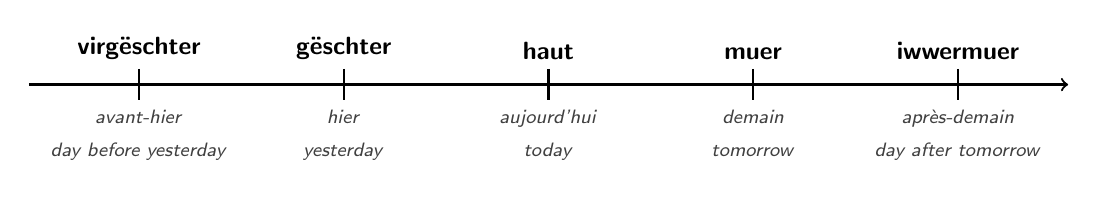
\begin{tikzpicture}[every node/.style={align=center, font=\sffamily}, scale=1.0]
    % Draw timeline
    \draw[thick, ->] (-6.6,0) -- (6.6,0);
    
    % virgëschter (-5.2)
    \draw[thick] (-5.2,0.2) -- (-5.2,-0.2);
    \node[above=0.2cm] at (-5.2,0) {\small\bfseries virgëschter};
    \node[below=0.2cm, text=black!75] at (-5.2,0) {\scriptsize\textit{avant-hier} \\ \scriptsize\textit{day before yesterday}};

    % gëschter (-2.6)
    \draw[thick] (-2.6,0.2) -- (-2.6,-0.2);
    \node[above=0.2cm] at (-2.6,0) {\small\bfseries gëschter};
    \node[below=0.2cm, text=black!75] at (-2.6,0) {\scriptsize\textit{hier} \\ \scriptsize\textit{yesterday}};

    % haut (0.0)
    \draw[thick] (0,0.2) -- (0,-0.2);
    \node[above=0.2cm] at (0,0) {\small\bfseries haut};
    \node[below=0.2cm, text=black!75] at (0,0) {\scriptsize\textit{aujourd'hui} \\ \scriptsize\textit{today}};

    % muer (2.6)
    \draw[thick] (2.6,0.2) -- (2.6,-0.2);
    \node[above=0.2cm] at (2.6,0) {\small\bfseries muer};
    \node[below=0.2cm, text=black!75] at (2.6,0) {\scriptsize\textit{demain} \\ \scriptsize\textit{tomorrow}};

    % iwwermuer (5.2)
    \draw[thick] (5.2,0.2) -- (5.2,-0.2);
    \node[above=0.2cm] at (5.2,0) {\small\bfseries iwwermuer};
    \node[below=0.2cm, text=black!75] at (5.2,0) {\scriptsize\textit{après-demain} \\ \scriptsize\textit{day after tomorrow}};
\end{tikzpicture}
\end{center}

\begin{itemize}
    \item \textbf{virgëschter} (oder \textbf{virugëschter}) : avant-hier / the day before yesterday. \\
    \textit{Virgëschter hunn ech de ganzen Dag geschafft.} \\
    $\rightarrow$ \textit{FR :} Avant-hier, j'ai travaillé toute la journée. \\
    $\rightarrow$ \textit{EN :} The day before yesterday, I worked all day long.

    \item \textbf{gëschter} : hier / yesterday. \\
    \textit{Gëschter war ech an der Stad.} \\
    $\rightarrow$ \textit{FR :} Hier, j'étais en ville. \\
    $\rightarrow$ \textit{EN :} Yesterday, I was in the city.

    \item \textbf{haut} : aujourd'hui / today. \\
    \textit{Haut ass e schéinen Dag.} \\
    $\rightarrow$ \textit{FR :} Aujourd'hui est une belle journée. \\
    $\rightarrow$ \textit{EN :} Today is a beautiful day.

    \item \textbf{muer} : demain / tomorrow. \\
    \textit{Muer hunn ech Congé.} \\
    $\rightarrow$ \textit{FR :} Demain, je suis en congé / j'ai un jour de repos. \\
    $\rightarrow$ \textit{EN :} Tomorrow, I have a day off.

    \item \textbf{iwwermuer} : après-demain / the day after tomorrow. \\
    \textit{Iwwermuer ginn ech op de Maart.} \\
    $\rightarrow$ \textit{FR :} Après-demain, je vais au marché. \\
    $\rightarrow$ \textit{EN :} The day after tomorrow, I am going to the market.
\end{itemize}

\subsection{D'Zukunft am geschwatenen Lëtzebuergesch (Kee Futur !) / L'expression du futur à l'oral / Expressing the Future in Spoken Luxembourgish}

En interessante linguistesche Punkt aus dem Cours : \\
\textbf{\flqq Lëtzebuergesch huet kee Futur, awer et huet eng Zukunft !\frqq} \\
\textit{FR : Le luxembourgeois n'a pas de temps futur formel, mais il a un avenir !} \\
\textit{EN : Luxembourgish has no formal future tense, but it has a future!}

Am Alldag gëtt de Futur quasi ni mat dem Hëllefsverb \textit{wäert} gebilt. Amplaz benotzt een einfach de \textbf{Präsens mat engem Zäitadverb} : \\
\textit{FR : Au quotidien, le futur n'est presque jamais formé avec l'auxiliaire \textit{wäert}. À la place, on emploie simplement le \textbf{présent accompagné d'un adverbe temporel} :} \\
\textit{EN : In everyday speech, the future is rarely formed with the auxiliary \textit{wäert}. Instead, one simply uses the \textbf{present tense combined with a time adverb}:}

\begin{itemize}
    \item \textit{Français :} \flqq Je serai là après-demain.\frqq \\
    $\rightarrow$ \textbf{Lëtzebuergesch :} \textbf{Ech sinn do iwwermuer.} (oder : \textbf{Iwwermuer sinn ech do.}) \\
    $\rightarrow$ \textit{EN :} I will be there the day after tomorrow.
    \item \textit{Français :} \flqq Demain, nous irons au concert.\frqq \\
    $\rightarrow$ \textbf{Lëtzebuergesch :} \textbf{Muer gi mir an de Concert.} \\
    $\rightarrow$ \textit{EN :} Tomorrow we are going to the concert.
\end{itemize}

\subsection{Lokaladverben : \textit{hei} vs. \textit{do} / Adverbes de lieu / Spatial Adverbs}
\begin{itemize}
    \item \textbf{hei} : ici (près du locuteur / here). \\
    \textit{Ech sinn hei.} $\rightarrow$ \textit{FR :} Je suis ici. / \textit{EN :} I am here.
    \item \textbf{do} : là / là-bas (éloigné du locuteur / there). \\
    \textit{Ech war do déi lescht Woch.} $\rightarrow$ \textit{FR :} J'étais là-bas la semaine dernière. / \textit{EN :} I was there last week.
\end{itemize}

\vspace{1.5em}

% ==============================================================================
% SECTION VI: NEGATIOUNEN AN D'EIFELER REGEL
% ==============================================================================
\section[Negatiounen an d'Eifeler Regel / Negation and the Eifeler Regel]{Negatiounen an d'Eifeler Regel \\/ Les trois négations et la règle de l'Eifel \\/ Negation Forms and the Eifeler Regel}

\subsection{Déi dräi Negatiounsformen am Verglach / Comparaison des négations / Comparison of Negations}

\begin{table}[htbp]
    \centering
    \begin{tabular}{p{2.6cm}p{4.0cm}p{8.5cm}}
        \toprule
        \textbf{Negatioun} & \textbf{Funktioun} & \textbf{Beispiller} \\
        \midrule
        \textbf{net} & Negéiert Verben, Adjektiver, Adverben & $\bullet$ \textit{Ech kann haut \textbf{net} kommen.} \newline $\rightarrow$ \textit{FR :} Je ne peux pas venir aujourd'hui. \newline $\rightarrow$ \textit{EN :} I cannot come today. \newline $\bullet$ \textit{D'Musek ass \textbf{net} haart.} \newline $\rightarrow$ \textit{FR :} La musique n'est pas forte. \newline $\rightarrow$ \textit{EN :} The music is not loud. \newline $\bullet$ \textit{Hie fiert \textbf{net} séier.} \newline $\rightarrow$ \textit{FR :} Il ne roule pas vite. \newline $\rightarrow$ \textit{EN :} He does not drive fast. \\
        \midrule
        \textbf{kee / keng / kee} & Negéiert Substantiver mat onbestëmmtem oder ouni Artikel & $\bullet$ \textit{Ech hu \textbf{keng} Zäit.} \newline $\rightarrow$ \textit{FR :} Je n'ai pas le temps. \newline $\rightarrow$ \textit{EN :} I have no time. \newline $\bullet$ \textit{Ech spillen \textbf{keen} Instrument.} \newline $\rightarrow$ \textit{FR :} Je ne joue d'aucun instrument. \newline $\rightarrow$ \textit{EN :} I do not play any instrument. \newline $\bullet$ \textit{Dat ass \textbf{kee} Problem.} \newline $\rightarrow$ \textit{FR :} Ce n'est pas un problème. \newline $\rightarrow$ \textit{EN :} That is no problem. \\
        \midrule
        \textbf{näischt} & Indefinitpronomen fir \flqq rien / nothing\frqq & $\bullet$ \textit{Ech hu gëschter \textbf{näischt} verstanen.} \newline $\rightarrow$ \textit{FR :} Je n'ai rien compris hier. \newline $\rightarrow$ \textit{EN :} I didn't understand anything yesterday. \newline $\bullet$ \textit{Mir hunn \textbf{näischt} héiert.} \newline $\rightarrow$ \textit{FR :} Nous n'avons rien entendu. \newline $\rightarrow$ \textit{EN :} We didn't hear anything. \\
        \bottomrule
    \end{tabular}
    \caption{Verglach tëscht \textit{net}, \textit{kee/keng} an \textit{näischt}}
\end{table}

\subsection{D'Eifeler Regel (N-Reegel) an der Praxis / La règle de l'Eifel en pratique / The Eifeler Regel in Practice}

D'Reegel seet : De Buschtaf \textbf{-n} (oder \textbf{-nn}) um Enn vun engem Wuert fällt ewech, \textbf{ausser} dat nächst Wuert fänkt un mat : \\
\textit{FR : La règle stipule que le \textbf{-n} (ou \textbf{-nn}) final d'un mot tombe, \textbf{sauf} si le mot suivant commence par :} \\
\textit{EN : The rule states that final \textbf{-n} (or \textbf{-nn}) drops, \textbf{unless} the following word begins with:}
\begin{center}
    \textbf{engem Vokal (A, E, I, O, U) \quad ODER \quad den Konsonanten D, T, Z, H}
\end{center}

\textit{Mnemonic aus dem Cours :} D'Konsonanten \textbf{D, T, Z, H} + Vokaler (United Saachen) halen den \textbf{-n} fest !

\begin{itemize}
    \item \textbf{Beispiller wou den -n bleift / Exemples où le -n est conservé / Examples where -n is kept :}
    \begin{itemize}
        \item \textit{kee\textbf{n} \textbf{H}unneg} (virun \textbf{H}) $\rightarrow$ \textit{FR :} pas de miel / \textit{EN :} no honey.
        \item \textit{kee\textbf{n} \textbf{I}nstrument} (virun engem Vokal \textbf{I}) $\rightarrow$ \textit{FR :} aucun instrument / \textit{EN :} no instrument.
        \item \textit{an enge\textbf{m} Concert} (Dativ Maskulin, bleift -m) $\rightarrow$ \textit{FR :} à un concert / \textit{EN :} at a concert.
        \item \textit{déi lesch\textbf{t} Kéier} (-t fält net ewech) $\rightarrow$ \textit{FR :} la dernière fois / \textit{EN :} the last time.
    \end{itemize}
    \item \textbf{Beispiller wou den -n ewechfält / Exemples où le -n tombe / Examples where -n drops :}
    \begin{itemize}
        \item \textit{kee\_ \textbf{P}roblem} (virun \textbf{P}) $\rightarrow$ \textit{FR :} pas de problème / \textit{EN :} no problem (net: \textit{\flqq keen Problem\frqq}).
        \item \textit{kee\_ \textbf{B}illjee} (virun \textbf{B}) $\rightarrow$ \textit{FR :} pas de billet / \textit{EN :} no ticket.
        \item \textit{mir spille\_ \textbf{G}ittar} (virun \textbf{G}) $\rightarrow$ \textit{FR :} nous jouons de la guitare / \textit{EN :} we play guitar.
    \end{itemize}
\end{itemize}

\vspace{1.5em}

% ==============================================================================
% SECTION VII: SPROOCHENTEST VIRBEREEDUNG (THEMA MUSEK)
% ==============================================================================
\section[Sproochentest Virbereedung: D'Thema Musek / Sproochentest Oral Prep]{Sproochentest Virbereedung : D'Thema Musek \\/ Préparation à l'épreuve orale : La Musique \\/ Sproochentest Oral Exam Preparation: Music}

\subsection{Deel 1 : Typesch Froen vum Examinateur a Musteräntwerten}

\begin{enumerate}
    \item \textbf{Examinateur :} \textit{Lauschtert Dir gäre Musek ? Wat fir eng Musek lauschtert Dir ?} \\
    $\rightarrow$ \textit{FR :} Aimez-vous écouter de la musique ? Quel genre de musique écoutez-vous ? \\
    $\rightarrow$ \textit{EN :} Do you like listening to music? What kind of music do you listen to? \\
    \textbf{Kandidat :} \textit{Jo, ech lauschtere ganz gäre Musek. Am léifste lauschteren ech klassesch Musek a Popmusek, well dat mech berouegt an entspaant. Moies beim Kaffisdrénken oder am Auto maachen ech ëmmer de Radio un. Wann ech kachen, lauschteren ech och gär lieweg Musek, heiansdo danzen ech souguer dobäi !} \\
    $\rightarrow$ \textit{FR :} Oui, j'aime beaucoup écouter de la musique. Ce que je préfère écouter, c'est la musique classique et la pop, car cela me calme et me détend. Le matin en prenant mon café ou dans la voiture, j'allume toujours la radio. Quand je cuisine, j'aime aussi écouter de la musique entraînante, parfois même je danse en cuisinant ! \\
    $\rightarrow$ \textit{EN :} Yes, I really like listening to music. What I prefer listening to is classical and pop music, because it calms and relaxes me. In the morning while having coffee or in the car, I always turn on the radio. When I cook, I also like listening to lively music, sometimes I even dance while cooking!
    
    \vspace{0.4em}

    \item \textbf{Examinateur :} \textit{Spillt Dir e Museksinstrument ? Hutt Dir fréier eppes gespillt ?} \\
    $\rightarrow$ \textit{FR :} Jouez-vous d'un instrument de musique ? En avez-vous joué par le passé ? \\
    $\rightarrow$ \textit{EN :} Do you play a musical instrument? Did you play anything previously? \\
    \textbf{Kandidat :} \textit{Haut spillen ech leider kee Museksinstrument méi, well ech net genuch Zäit dofir hunn. Awer wéi ech jonk war, hunn ech ongeféier fënnef Joer laang Gittar gespillt. Meng Elteren haten och e Piano doheem, an ech hunn e bësse probéiert ze spillen. Wann ech méi Zäit hätt, géif ech gär erëm mat der Gittar ufänken.} \\
    $\rightarrow$ \textit{FR :} Aujourd'hui, je ne joue malheureusement plus d'aucun instrument de musique parce que je n'ai pas assez de temps pour cela. Mais quand j'étais jeune, j'ai joué de la guitare pendant environ cinq ans. Mes parents avaient aussi un piano à la maison, et j'ai un peu essayé d'en jouer. Si j'avais plus de temps, j'aimerais bien recommencer la guitare. \\
    $\rightarrow$ \textit{EN :} Today, unfortunately, I no longer play any musical instrument because I don't have enough time for it. But when I was young, I played guitar for about five years. My parents also had a piano at home, and I tried playing a bit. If I had more time, I would gladly start playing guitar again.

    \vspace{0.4em}

    \item \textbf{Examinateur :} \textit{Gitt Dir dacks op Concerten oder Festivaller ?} \\
    $\rightarrow$ \textit{FR :} Allez-vous souvent à des concerts ou des festivals ? \\
    $\rightarrow$ \textit{EN :} Do you often go to concerts or festivals? \\
    \textbf{Kandidat :} \textit{Jo, ech ginn zimmlech gär op Concerten. Déi lescht Kéier war ech an der Philharmonie um Kierchbierg, fir e klassesche Concert ze kucken. D'Akustik do ass wierklech fantastesch. Am Summer ginn ech och gäre mat Frënn op d'Fête de la Musique an der Stad oder op de Blues'n Jazz Rallye am Gronn. Do ass ëmmer eng flott a gemittlech Ambiance.} \\
    $\rightarrow$ \textit{FR :} Oui, j'aime assez aller à des concerts. La dernière fois, j'étais à la Philharmonie au Kirchberg pour voir un concert classique. L'acoustique y est vraiment fantastique. En été, je vais aussi volontiers avec des amis à la Fête de la Musique en ville ou au Blues'n Jazz Rallye dans le Grund. Il y règne toujours une ambiance agréable et conviviale. \\
    $\rightarrow$ \textit{EN :} Yes, I quite like going to concerts. Last time, I was at the Philharmonie on the Kirchberg to see a classical concert. The acoustics there are truly fantastic. In the summer, I also gladly go with friends to the Fête de la Musique in the city or to the Blues'n Jazz Rallye in the Grund. There is always a wonderful and cozy atmosphere there.

    \vspace{0.4em}

    \item \textbf{Examinateur :} \textit{Gëtt et eng Musek, déi Dir guer net gär hutt ?} \\
    $\rightarrow$ \textit{FR :} Y a-t-il un genre de musique que vous n'aimez pas du tout ? \\
    $\rightarrow$ \textit{EN :} Is there any music that you do not like at all? \\
    \textbf{Kandidat :} \textit{Jo, ech hu guer kee schwéiere Rock oder Heavy Metal gär. Dat ass mir einfach ze haart an ze hektesch. Wann ech sou eng Musek lauschteren, ginn ech nervos an ech langweilen mech séier.} \\
    $\rightarrow$ \textit{FR :} Oui, je n'aime pas du tout le rock lourd ou le heavy metal. C'est tout simplement trop fort et trop agité pour moi. Quand j'écoute ce genre de musique, je deviens nerveux et je m'ennuie rapidement. \\
    $\rightarrow$ \textit{EN :} Yes, I don't like heavy rock or heavy metal at all. It is simply too loud and too hectic for me. When I listen to such music, I get nervous and I quickly get bored.
\end{enumerate}

\subsection{Deel 2 : Bildbeschreiwung (Bild mat Museker / Concert) / Description d'image / Picture Description}

Eng klassesch Aufgab am Sproochentest ass d'Beschreiwung vun engem Bild. Hei ass e strukturéierte Modell fir e Concerts- oder Museksbild mat Iwwersetzungen : \\
\textit{FR : Une épreuve classique du Sproochentest est la description d'une image. Voici un modèle structuré pour une scène de concert ou de répétition musicale :} \\
\textit{EN : A standard task in the Sproochentest is the description of an image. Here is a structured model for a concert or musical rehearsal scene:}

\begin{center}
    \framebox{\parbox{0.92\linewidth}{\centering
        \vspace{0.2cm}
        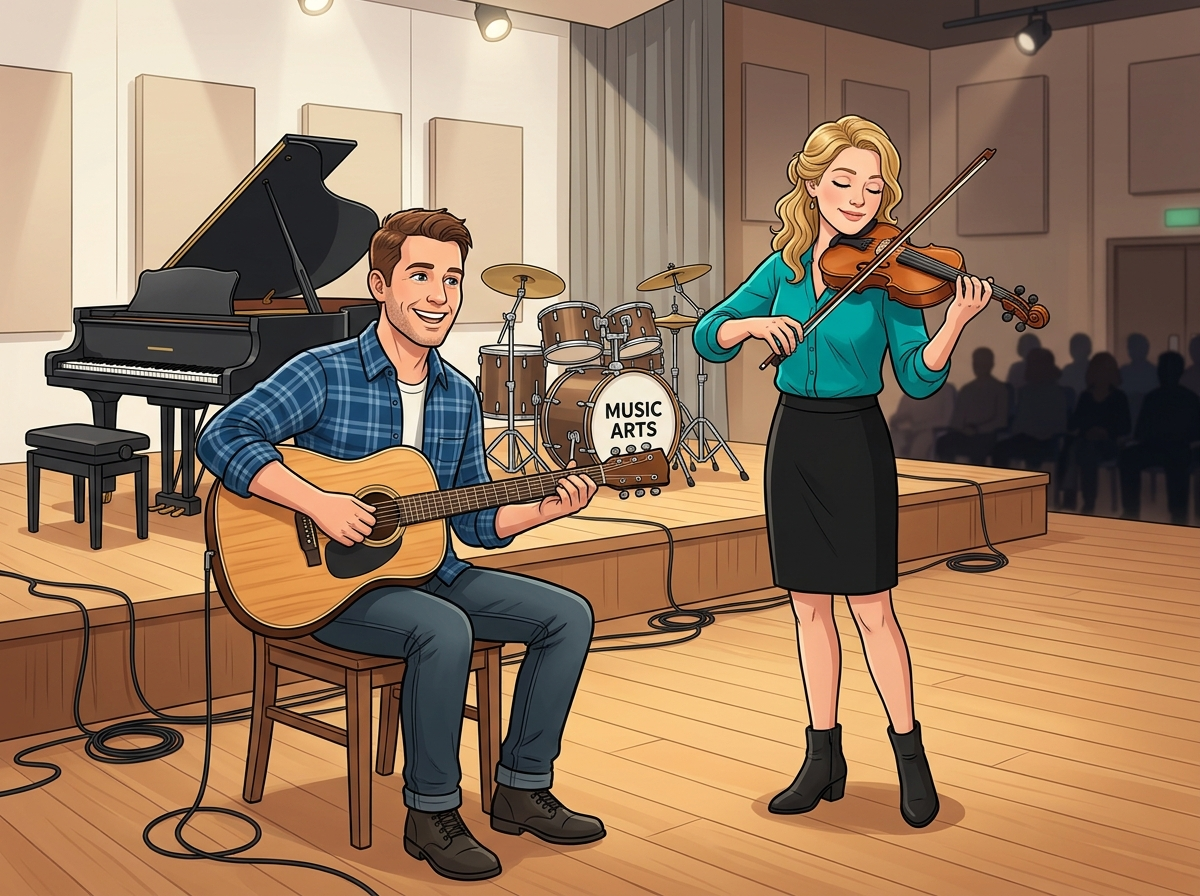
\includegraphics[width=0.88\linewidth]{vokab_300dpi/concert_ensembel.png} \\
        \vspace{0.2cm}
        \small\textbf{Musterbild fir de Sproochentest : E klenge Museksensembel op der Bühn} \\
        \footnotesize\textit{(FR : Image modèle pour le Sproochentest : Petit ensemble musical sur scène / EN : Sample image for the Sproochentest: Small musical ensemble on stage)}
    }}
\end{center}

\vspace{0.6em}

\begin{itemize}
    \item \textbf{Allgemengen Androck / Impression générale / General Impression :} \\
    \textit{Op dësem Bild gesinn ech eng Grupp vu Leit, déi Musek maachen. Et gesäit aus wéi e Concert oder eng Prouf vun engem klenge Museksensembel.} \\
    $\rightarrow$ \textit{FR :} Sur cette image, je vois un groupe de personnes qui font de la musique. Cela ressemble à un concert ou à une répétition d'un petit ensemble musical. \\
    $\rightarrow$ \textit{EN :} In this picture, I see a group of people making music. It looks like a concert or a rehearsal of a small musical ensemble.

    \vspace{0.3em}

    \item \textbf{Am Virdergrond / Au premier plan / In the foreground :} \\
    \textit{Am Virdergrond sëtzt e Mann, dee Gittar spillt. Hien huet eng akustesch Gittar a laacht. Nieft him steet eng Fra, déi Gei spillt. Si huet d'Aen zou a konzentréiert sech ganz op d'Musek.} \\
    $\rightarrow$ \textit{FR :} Au premier plan, un homme est assis et joue de la guitare. Il a une guitare acoustique et sourit. À côté de lui se tient une femme qui joue du violon. Elle a les yeux fermés et se concentre pleinement sur la musique. \\
    $\rightarrow$ \textit{EN :} In the foreground sits a man who is playing guitar. He has an acoustic guitar and is smiling. Beside him stands a woman playing the violin. Her eyes are closed and she is concentrating fully on the music.

    \vspace{0.3em}

    \item \textbf{Am Hannergrond / À l'arrière-plan / In the background :} \\
    \textit{Am Hannergrond gesäit een e Piano an eng Batterie. D'Leit am Publikum klappen an d'Hänn a freeën sech.} \\
    $\rightarrow$ \textit{FR :} À l'arrière-plan, on aperçoit un piano et une batterie. Les personnes dans le public applaudissent et ont l'air réjouies. \\
    $\rightarrow$ \textit{EN :} In the background, one can see a piano and drums. The people in the audience are clapping and looking cheerful.

    \vspace{0.3em}

    \item \textbf{Perséinlech Meenung / Opinion personnelle / Personal Opinion :} \\
    \textit{D'Ambiance um Bild wierkt ganz waarm, freedeg an harmonesch. Ech mengen, d'Leit hunn e ganz flotten Owend zesummen.} \\
    $\rightarrow$ \textit{FR :} L'ambiance sur l'image semble très chaleureuse, joyeuse et harmonieuse. Je pense que les gens passent une excellente soirée ensemble. \\
    $\rightarrow$ \textit{EN :} The atmosphere in the picture seems very warm, joyful, and harmonious. I think the people are having a wonderful evening together.
\end{itemize}

\vspace{1.5em}

% ==============================================================================
% SECTION VIII: ÜBUNGEN A LÉISUNGEN
% ==============================================================================
\section[Übungen a Léisungen / Exercises and Solutions]{Übungen a Léisungen \\/ Exercices et solutions \\/ Exercises and Solutions}

\subsection*{Übung 1 : Fëllt d'Lücken aus (Musek a Prepositiounen)}
\textit{Setzt déi richteg Wierder an : \textbf{an engem}, \textbf{op engem}, \textbf{Wat fir eng}, \textbf{eppes}, \textbf{keen}, \textbf{keng}, \textbf{lauschteren}, \textbf{héieren}.} \\
\textit{\small(FR : Remplissez les trous avec les mots ci-dessus / EN : Fill in the blanks with the words above)}

\begin{enumerate}
    \item \underline{\hspace{3cm}} Musek lauschters du am léifsten ? \\
    \small\textit{(FR : Quel genre de musique écoutes-tu de préférence ? / EN : What kind of music do you like to listen to best?)}
    \item Ech spillen leider \underline{\hspace{2.5cm}} Instrument, mee ech lauschtere gär Musek. \\
    \small\textit{(FR : Malheureusement je ne joue d'aucun instrument... / EN : Unfortunately I don't play any instrument...)}
    \item Mir waren de Weekend \underline{\hspace{3cm}} Concert an der Philharmonie. \\
    \small\textit{(FR : Nous étions ce week-end à un concert... / EN : We were at a concert this weekend...)}
    \item Si huet gëschter \underline{\hspace{3cm}} Festival am Fräie vill gedanzt. \\
    \small\textit{(FR : Elle a beaucoup dansé hier à un festival... / EN : She danced a lot yesterday at a festival...)}
    \item Kanns du wgl. roueg sinn ? Ech wëll \underline{\hspace{2.5cm}} um Radio \underline{\hspace{2.5cm}}. \\
    \small\textit{(FR : Peux-tu être calme s'il te plaît ? Je veux écouter quelque chose... / EN : Can you please be quiet? I want to listen to something...)}
    \item Ech hu momentan \underline{\hspace{2.5cm}} Zäit fir an de Concert ze goen. \\
    \small\textit{(FR : Je n'ai pas le temps en ce moment d'aller au concert... / EN : I currently have no time to go to a concert...)}
\end{enumerate}

\subsection*{Übung 2 : Modalverben am Präteritum}
\textit{Konjugéiert d'Verb am Präteritum (Imparfait) :} \\
\textit{\small(FR : Conjuguez le verbe modal au prétérit / EN : Conjugate the modal verb in the preterite)}

\begin{enumerate}
    \item Gëschter (\textit{kënnen}) ech net an de Cours kommen, well ech krank war. \\
    \small\textit{(FR : Hier, je n'ai pas pu venir au cours parce que j'étais malade / EN : Yesterday, I could not come to class because I was sick)}
    \item Mir (\textit{wëllen}) e Billjee fir d'Rockhal kafen, mee et waren der keng méi do. \\
    \small\textit{(FR : Nous voulions acheter un billet pour la Rockhal... / EN : We wanted to buy a ticket for the Rockhal...)}
    \item Hien (\textit{mussen}) de ganzen Dag am Büro bleiwen. \\
    \small\textit{(FR : Il a dû rester toute la journée au bureau / EN : He had to stay at the office all day)}
    \item (\textit{wëssen}) dir, datt d'Adele e Concert zu Lëtzebuerg gëtt ? \\
    \small\textit{(FR : Saviez-vous qu'Adele donne un concert au Luxembourg ? / EN : Did you know that Adele gives a concert in Luxembourg?)}
    \item D'Kanner (\textit{dierfen}) fréier net ouni d'Elteren an de Kino goen. \\
    \small\textit{(FR : Autrefois, les enfants n'avaient pas le droit d'aller au cinéma... / EN : In the past, children were not allowed to go to the cinema...)}
    \item Ech (\textit{sollen}) mäi Frënd uruffen, mee ech hu mäin Handy vergiess. \\
    \small\textit{(FR : Je devais appeler mon ami, mais j'ai oublié mon portable / EN : I was supposed to call my friend, but I forgot my mobile phone)}
\end{enumerate}

\subsection*{Übung 3 : Sazbau an Inversioun (Franséisch op Lëtzebuergesch)}
\textit{Iwwersetzt dës Sätz op Lëtzebuergesch a passt op d'Wuertstellung an d'Inversioun op :} \\
\textit{\small(FR : Traduisez ces phrases en luxembourgeois en faisant attention à l'ordre des mots et à l'inversion / EN : Translate these sentences into Luxembourgish paying attention to word order and inversion)}

\begin{enumerate}
    \item Quand j'écoute de la bonne musique, je suis de bonne humeur. \\
    \small\textit{(EN : When I listen to good music, I am in a good mood)}
    \item Malheureusement, je n'ai pas le temps de jouer de la guitare. \\
    \small\textit{(EN : Unfortunately, I don't have time to play guitar)}
    \item Demain, nous irons à Luxembourg-Ville pour acheter un piano. \\
    \small\textit{(EN : Tomorrow we will go to Luxembourg City to buy a piano)}
    \item Quand tu t'ennuies, tu écoutes la radio. \\
    \small\textit{(EN : When you get bored, you listen to the radio)}
    \item Je serai là après-demain pour le concert. \\
    \small\textit{(EN : I will be there the day after tomorrow for the concert)}
\end{enumerate}

\vspace{1em}

\subsection*{Léisunge fir d'Übungen}

\subsubsection*{Léisung fir Übung 1}
\begin{enumerate}
    \item \textbf{Wat fir eng} Musek lauschters du am léifsten ? \\
    $\rightarrow$ \textit{FR :} Quel genre de musique écoutes-tu de préférence ? / \textit{EN :} What kind of music do you like to listen to best?
    \item Ech spillen leider \textbf{keen} Instrument, mee ech lauschtere gär Musek. \\
    $\rightarrow$ \textit{FR :} Malheureusement je ne joue d'aucun instrument, mais j'aime écouter de la musique. / \textit{EN :} Unfortunately I don't play any instrument, but I like listening to music.
    \item Mir waren de Weekend \textbf{an engem} Concert an der Philharmonie. \\
    $\rightarrow$ \textit{FR :} Nous étions ce week-end à un concert à la Philharmonie. / \textit{EN :} We were at a concert at the Philharmonie this weekend.
    \item Si huet gëschter \textbf{op engem} Festival am Fräie vill gedanzt. \\
    $\rightarrow$ \textit{FR :} Elle a beaucoup dansé hier à un festival en plein air. / \textit{EN :} She danced a lot yesterday at an open-air festival.
    \item Kanns du wgl. roueg sinn ? Ech wëll \textbf{eppes} um Radio \textbf{lauschteren}. \\
    $\rightarrow$ \textit{FR :} Peux-tu être calme s'il te plaît ? Je veux écouter quelque chose à la radio. / \textit{EN :} Can you please be quiet? I want to listen to something on the radio.
    \item Ech hu momentan \textbf{keng} Zäit fir an de Concert ze goen. \\
    $\rightarrow$ \textit{FR :} Je n'ai pas le temps en ce moment d'aller au concert. / \textit{EN :} I currently have no time to go to a concert.
\end{enumerate}

\subsubsection*{Léisung fir Übung 2}
\begin{enumerate}
    \item Gëschter \textbf{konnt} ech net an de Cours kommen, well ech krank war. \\
    $\rightarrow$ \textit{FR :} Hier je n'ai pas pu venir au cours parce que j'étais malade. \\
    $\rightarrow$ \textit{EN :} Yesterday I could not come to class because I was sick.
    \item Mir \textbf{wollten} e Billjee fir d'Rockhal kafen, mee et waren der keng méi do. \\
    $\rightarrow$ \textit{FR :} Nous voulions acheter un billet pour la Rockhal, mais il n'y en avait plus. \\
    $\rightarrow$ \textit{EN :} We wanted to buy a ticket for the Rockhal, but there were none left.
    \item Hien \textbf{musst} de ganzen Dag am Büro bleiwen. \\
    $\rightarrow$ \textit{FR :} Il a dû rester toute la journée au bureau. \\
    $\rightarrow$ \textit{EN :} He had to stay at the office all day.
    \item \textbf{Wousst} dir, datt d'Adele e Concert zu Lëtzebuerg gëtt ? \\
    $\rightarrow$ \textit{FR :} Saviez-vous qu'Adele donne un concert au Luxembourg ? \\
    $\rightarrow$ \textit{EN :} Did you know that Adele is giving a concert in Luxembourg?
    \item D'Kanner \textbf{duerften} fréier net ouni d'Elteren an de Kino goen. \\
    $\rightarrow$ \textit{FR :} Autrefois, les enfants n'avaient pas le droit d'aller au cinéma sans leurs parents. \\
    $\rightarrow$ \textit{EN :} In the past, children were not allowed to go to the cinema without their parents.
    \item Ech \textbf{sollt} mäi Frënd uruffen, mee ech hu mäin Handy vergiess. \\
    $\rightarrow$ \textit{FR :} Je devais appeler mon ami, mais j'ai oublié mon téléphone portable. \\
    $\rightarrow$ \textit{EN :} I was supposed to call my friend, but I forgot my mobile phone.
\end{enumerate}

\subsubsection*{Léisung fir Übung 3}
\begin{enumerate}
    \item \textit{Français :} Quand j'écoute de la bonne musique, je suis de bonne humeur. \\
    $\rightarrow$ \textit{English :} When I listen to good music, I am in a good mood. \\
    $\rightarrow$ \textbf{Wann ech gutt Musek lauschteren, sinn ech gutt gelaunt.}
    \item \textit{Français :} Malheureusement, je n'ai pas le temps de jouer de la guitare. \\
    $\rightarrow$ \textit{English :} Unfortunately, I don't have time to play guitar. \\
    $\rightarrow$ \textbf{Leider hunn ech keng Zäit fir Gittar ze spillen.}
    \item \textit{Français :} Demain, nous irons à Luxembourg-Ville pour acheter un piano. \\
    $\rightarrow$ \textit{English :} Tomorrow we are going to Luxembourg City to buy a piano. \\
    $\rightarrow$ \textbf{Muer gi mir an d'Stad fir e Piano ze kafen.}
    \item \textit{Français :} Quand tu t'ennuies, tu écoutes la radio. \\
    $\rightarrow$ \textit{English :} When you get bored, you listen to the radio. \\
    $\rightarrow$ \textbf{Wann s de dech langweils, lauschters de de Radio.}
    \item \textit{Français :} Je serai là après-demain pour le concert. \\
    $\rightarrow$ \textit{English :} I will be there the day after tomorrow for the concert. \\
    $\rightarrow$ \textbf{Ech sinn do iwwermuer fir de Concert.} (oder : \textbf{Iwwermuer sinn ech do fir de Concert.})
\end{enumerate}

\vspace{2em}

% ==============================================================================
% SECTION IX: VOKABELEN MAT BILLER
% ==============================================================================
\section[Vokabelen mat Biller / Picture Dictionary]{Vokabelen mat Biller / Dictionnaire illustré / Illustrated Dictionary}

\begin{noindent}
\begin{minipage}[t]{0.48\textwidth}
    \centering
    \textbf{\Large Eng Gei}
    \vspace{0.4em}
    \framebox{\parbox{0.88\linewidth}{\centering
            \vspace{0.3cm}
            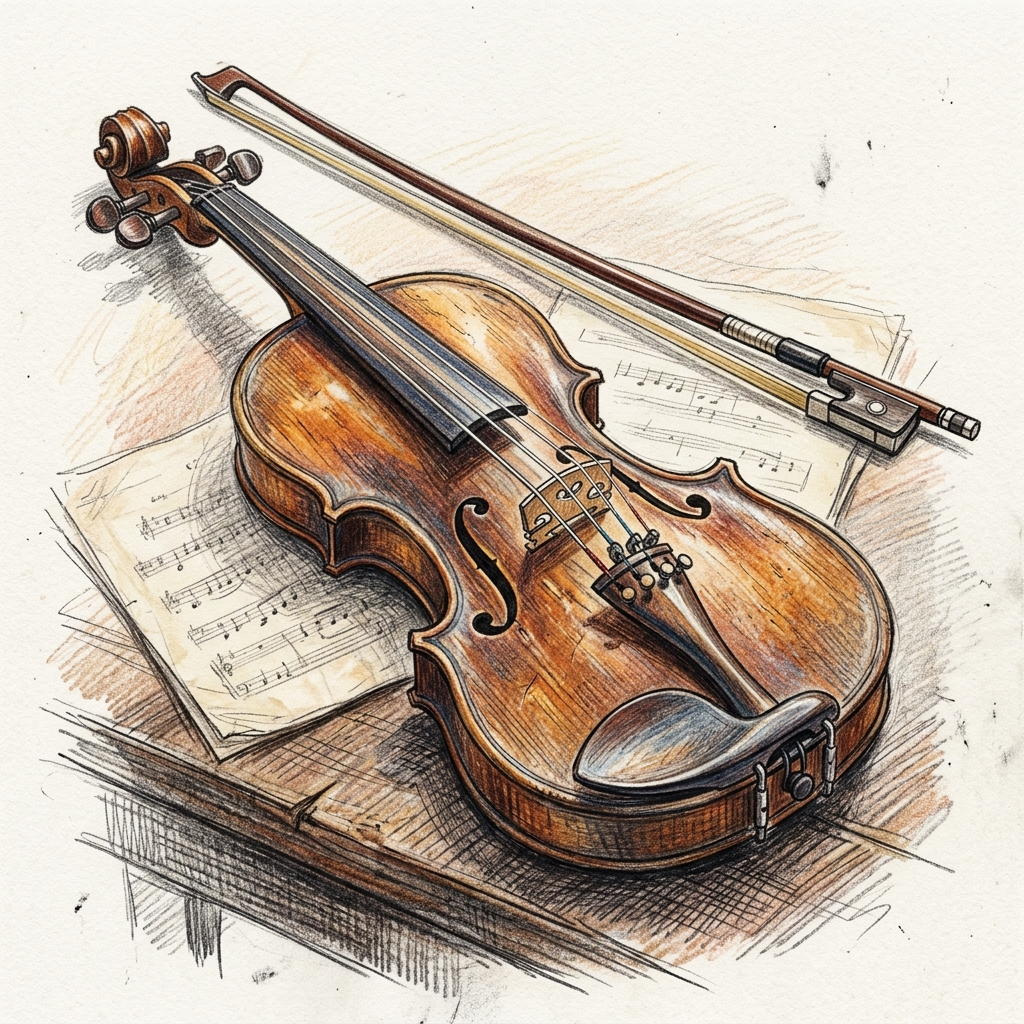
\includegraphics[width=0.85\linewidth]{vokab_300dpi/gei.png} \\
            \vspace{0.3cm}
    }}
    \vspace{0.4em}
    \textbf{\Large D'Gei}\\
    \small\textit{(Le violon / The violin)}
\end{minipage}
\hfill
\begin{minipage}[t]{0.48\textwidth}
    \centering
    \textbf{\Large Danzen}
    \vspace{0.4em}
    \framebox{\parbox{0.88\linewidth}{\centering
            \vspace{0.3cm}
            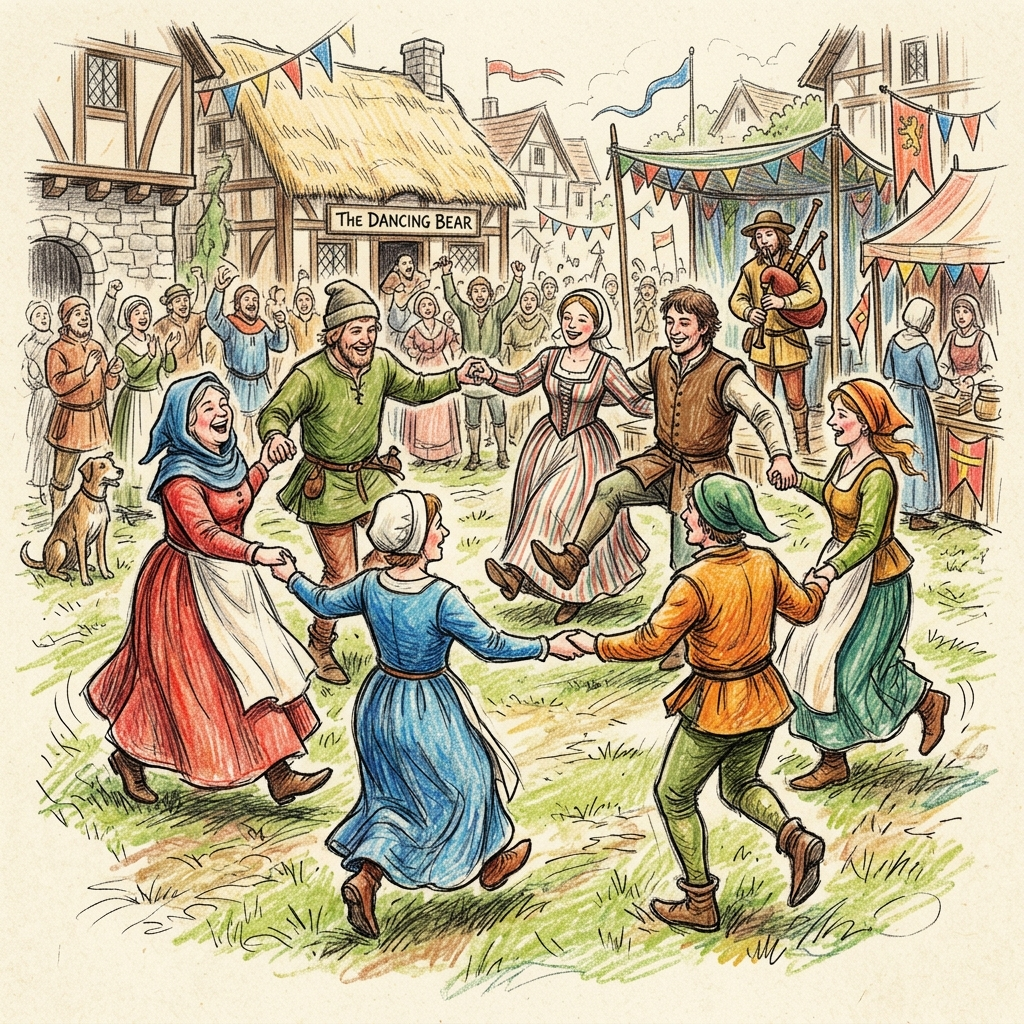
\includegraphics[width=0.85\linewidth]{vokab_300dpi/danzen.png} \\
            \vspace{0.3cm}
    }}
    \vspace{0.4em}
    \textbf{\Large Danzen (Danzkachen)}\\
    \small\textit{(Danser / To dance)}
\end{minipage}
\end{noindent}

\vspace{2em}

\begin{noindent}
\begin{minipage}[t]{0.48\textwidth}
    \centering
    \textbf{\Large Eng Gittar}
    \vspace{0.4em}
    \framebox{\parbox{0.88\linewidth}{\centering
            \vspace{0.3cm}
            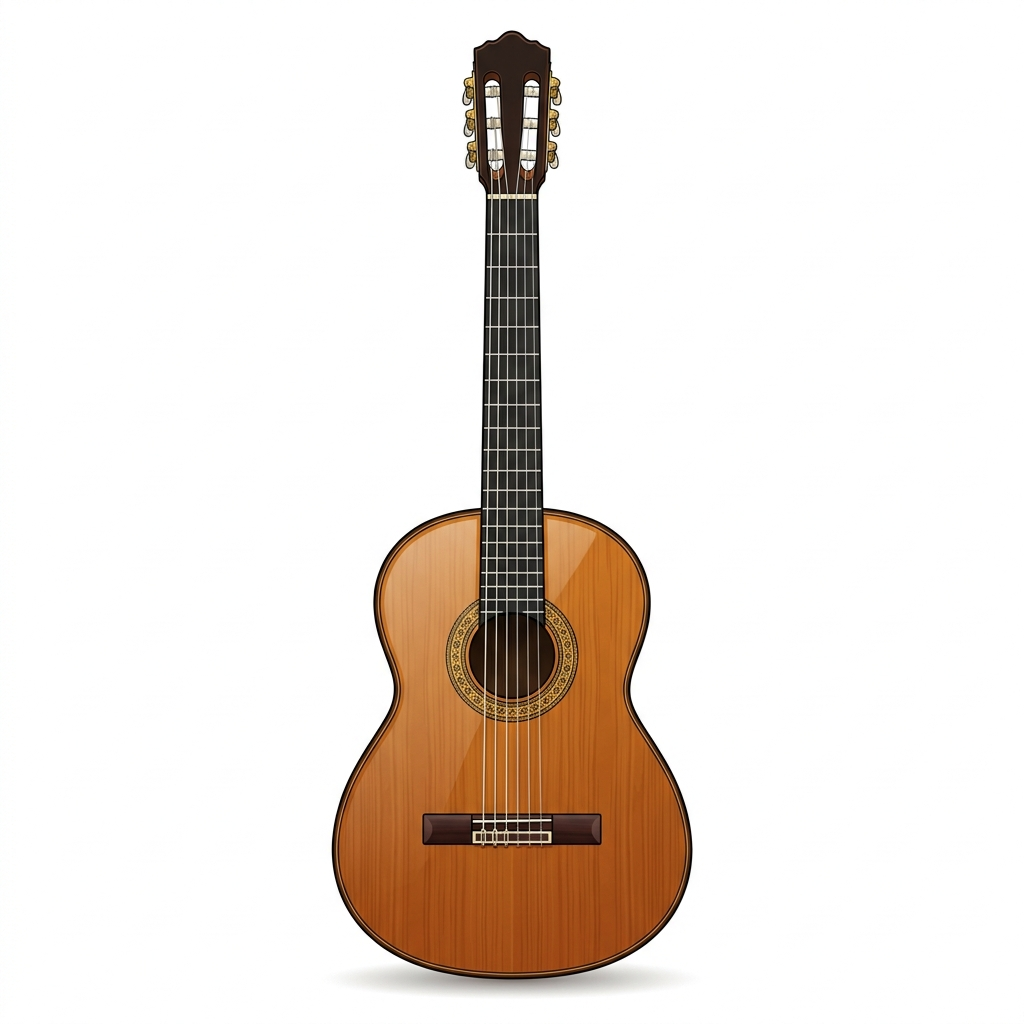
\includegraphics[width=0.85\linewidth]{vokab_300dpi/gittar.png} \\
            \vspace{0.3cm}
    }}
    \vspace{0.4em}
    \textbf{\Large D'Gittar}\\
    \small\textit{(La guitare / The guitar)}
\end{minipage}
\hfill
\begin{minipage}[t]{0.48\textwidth}
    \centering
    \textbf{\Large E Piano}
    \vspace{0.4em}
    \framebox{\parbox{0.88\linewidth}{\centering
            \vspace{0.3cm}
            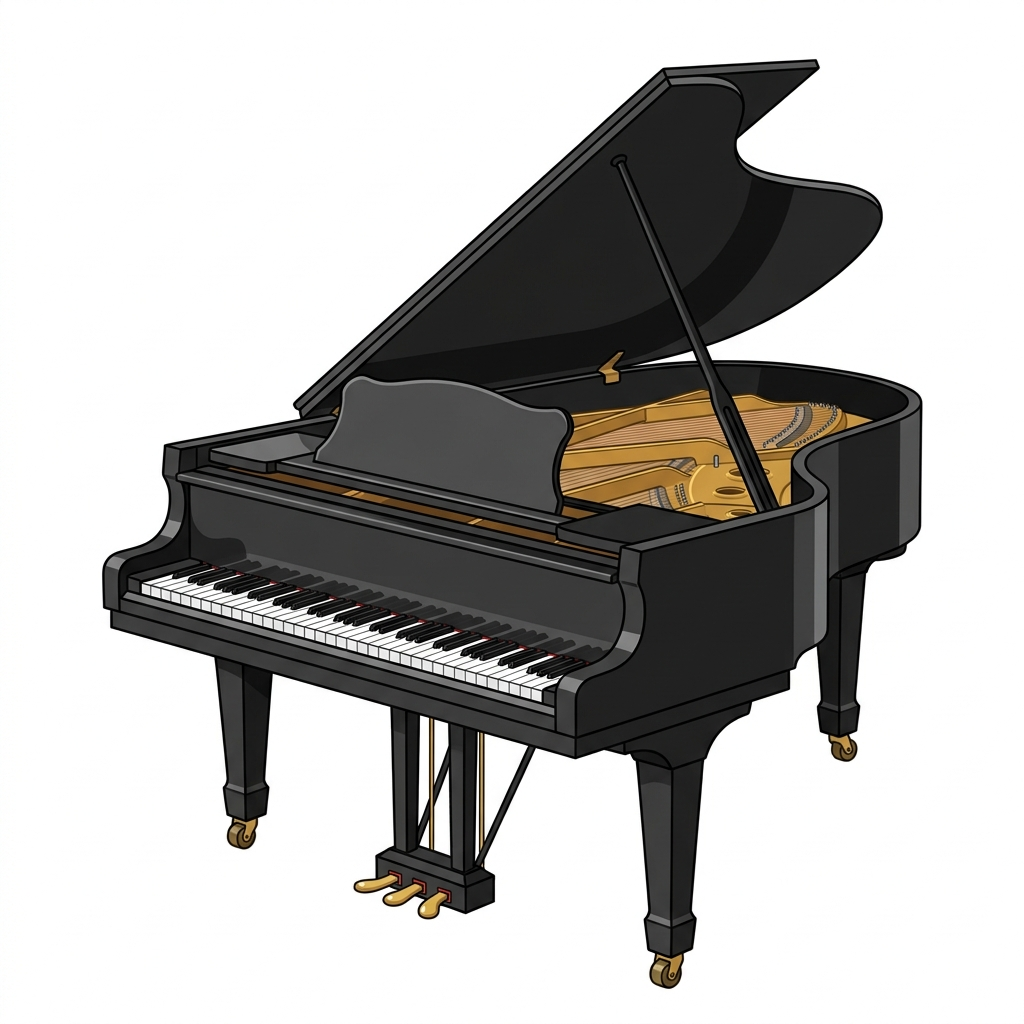
\includegraphics[width=0.85\linewidth]{vokab_300dpi/piano.png} \\
            \vspace{0.3cm}
    }}
    \vspace{0.4em}
    \textbf{\Large De Piano}\\
    \small\textit{(Le piano / The piano)}
\end{minipage}
\end{noindent}
